%!TEX root = ../thesis.tex
\chapter{Design \& Implementation}

	Development of a graphical user interface for libmapper creates a unique challenge. Obviously such an interface is a practical tool, and should function as such, yet it also must work in concert with DMIs which are inherently designed for creative use. For the purposes of this project, the assumed solution to this innate paradox is to provide the user with multiple independent modes of control.  This assumption based on experiences with prior user interfaces for libmapper: for each interface users reported excellent functionality for certain use cases, and poor functionality for others. libmapper itself is an extremely flexible API that makes few assumptions as to the network of devices and signals or how they are mapped. It is thus fitting that a GUI for libmapper would be equally as flexible. In lieu of a single perfect solution for network visualization and interactivity, providing users with various independent solutions provided a good compromise.

%%%%%%%%%%%%%%%%%%%%%%%%%%%%%%%%%%%%%%%%%%%%%%%%%%%%%%%%%%%%%%%%%%%%%%%%%%%%%%%%%%%%%%%%%%%%%%%%%%%%%%%%%%%%%%%%%%%%%%%%%%%%%%%%%%%%%%%%%%%%%%%%%%%%%%%%%%%%%%%%%%%%%%%%%%%%%%%%%%%%%%%%%%%%%%%%%%%%%%%%%%%%%%%%%%%%%%%%%%%%%%%%%%%%%%%%%%%%%%%%%%%%%%%%%%%%%%%%%%
\section{Prior interfaces for libmapepr} % (fold)
\label{sec:prior_interfaces_for_libmapepr}

	\subsection{Maxmapper} % (fold)
	\label{sub:maxmapper}
	
	% subsection maxmapper (end)

	\subsection{Vizmapper} % (fold)
	\label{sub:vizmapper}
	
	% subsection vizmapper (end)

	\subsection{Webmapper} % (fold)
	\label{sub:webmapper}
	
\begin{figure}[ht]
	\centering
	%\scalebox{0.42}{
	\includegraphics[width=1\textwidth]%
		{figures/webmapper}
	\caption{The webmapper interface}
	\label{fig:webmapper}
\end{figure}

Work on this project began with a moderately featured, little used GUI for libmapper known as ``webmapper.'' Webmapper was created at IDMIL as an attempt to replace the Max/MSP GUI as the result of limitations described in section \ref{sec:similar_interfaces}, the principle among which being the cross-platform incompatibility of Max/MSP. It was thought that a browser-based approach would greatly simplify the process of creating cross-compatibility with all major operating systems and even mobile devices. 

Webmapper utilizes the Python bindings for libmapper by registering an administrative monitor to communicate with a libmapper network. The monitor can create and modify connections or links, as well as query the network as to what devices, signals, links and connections are present. The webmapper code creates a simple HTTP server and attempts to open Google Chrome\footnote{Chrome Browser. [Online]. Available: \url{https://www.google.com/intl/en/chrome/browser/}. Accessed July 17, 2013} on the host computer. If Google Chrome is not present, the user must navigate directly to the server using the web address \url{localhost:50000}. The monitor communicates with the libmapper network and the local server, the browser is able to see messages the monitor ``posts'' to the server (such as `new device') and respond to them appropriately. The browser in turn can send messages to the server (like `connect') that will propagate up to libmapper itself, eventually resulting in a message cascading back down to the browser reflecting the change to the network (such as `new connection'). 

The interface itself is written for a web browser using the scripting language JavaScript\footnote{JavaScript | MDN. [Online]. Available: \url{https://developer.mozilla.org/en-US/docs/Web/JavaScript}. Accessed July 17, 2013} to control web-standard HyperText Markup Language (HTML) elements and Cascading Style Sheets (CSS). The JavaScript code stores four main data structures: devices, links, connections and signals. The code never directly modifies any of this data, and instead waits for messages relayed from libmapper. For example: if a user creates a new link, webmapper does not add the link directly to the links array but simply sends a message to the network. If it receives back a `new link' message, only then does it add the new link to the array. This is done to ensure that the data structures within webmapper always reflect what is actually present.

Figure \ref{fig:webmapper} displays the look of the interface before this project began. Users are able to perform all libmapper functions: connecting, linking and modifying connections, but only the simplest of feature sets is included. In order to form a connection the user must click on a source signal, click on a destination signal and then click on a button labeled ``connect.'' Many useful features of the Max/MSP interface, such as column headers, table sorting, drawing connections and search filtering are not present.

	% subsection webmapper (end)

% section prior_interfaces_for_libmapepr (end)


%%%%%%%%%%%%%%%%%%%%%%%%%%%%%%%%%%%%%%%%%%%%%%%%%%%%%%%%%%%%%%%%%%%%%%%%%%%%%%%%%%%%%%%%%%%%%%%%%%%%%%%%%%%%%%%%%%%%%%%%%%%%%%%%%%%%%%%%%%%%%%%%%%%%%%%%%%%%%%%%%%%%%%%%%%%%%%%%%%%%%%%%%%%%%%%%%%%%%%%%%%%%%%%%%%%%%%%%%%%%%%%%%%%%%%%%%%%%%%%%%%%%%%%%%%%%%%%%%%
\section{Integration of Interface Features}
	
	\subsection{Display libmapper metadata} % (fold)
	\label{sub:display_libmapper_metadata}
	
	% subsection display_libmapper_metadata (end)

	\subsection{Visual feedback} % (fold)
	\label{sub:visual_feedback}
		% # of signals/etc.
		% muted lines

	% subsection visual_feedback (end)

	\subsection{Namespace filtering} % (fold)
	\label{sub:namespace_filtering}
	
	% subsection namespace_filtering (end)

	\subsection{Table sorting} % (fold)
	\label{sub:table_sorting}
	
	% subsection table_sorting (end)

	\subsection{Draggable connections and links} % (fold)
	\label{sub:draggable_connections_and_links}
	
	% subsection draggable_connections_and_links (end)


%%%%%%%%%%%%%%%%%%%%%%%%%%%%%%%%%%%%%%%%%%%%%%%%%%%%%%%%%%%%%%%%%%%%%%%%%%%%%%%%%%%%%%%%%%%%%%%%%%%%%%%%%%%%%%%%%%%%%%%%%%%%%%%%%%%%%%%%%%%%%%%%%%%%%%%%%%%%%%%%%%%%%%%%%%%%%%%%%%%%%%%%%%%%%%%%%%%%%%%%%%%%%%%%%%%%%%%%%%%%%%%%%%%%%%%%%%%%%%%%%%%%%%%%%%%%%%%%%%
\section{Extension of Control and Visual Elements}

	\subsection{Evaluation of libmapper variables} % (fold)
	\label{sec:evaluation_of_libmapper_variables}

The list in table \ref{tab:metadata_types} is by no means a complete set, as libmapper may yet expand to include data like device position and users are able to tag devices/signals/links/connections with any extra data they may want.

A fourth data category \emph{boolean} has been added to specify data that only has two values (\emph{true or false}), as it is a common metadata feature. Boolean information is not covered in the Mackinlay paper. Going forward it will be treated more or less like ordinal data, as \emph{true} obviously has a relationship to \emph{false}, even though there is no quantitative value associated with them.


\begin{longtable}{l l l l}
\caption[libmapper metadata types]{libmapper metadata types} \label{tab:metadata_types} \\

	\hline\hline
	\textbf{Devices} & & \\
	\emph{quantitative} & \emph{ordinal} & \emph{nominal}\\
	\hline
	number of inputs & device ordinal & device name\\
		number of outputs \\
	ip address \\
	port \\ [0.7cm]

	\hline\hline
	\textbf{Signals} & & \\
	\emph{quantitative} & \emph{ordinal} & \emph{nominal}\\
	\hline
	length & direction & parent device name\\
	minimum value & & signal name \\
	maximum value & & data type (float, integer, etc.)\\
	sampling rate & & units \\ [0.7cm]

	\hline\hline
	\textbf{Links} & & \\
	\emph{quantitative} & \emph{ordinal} & \emph{nominal}\\
	\hline
	& & link name \\
	& & source device name \\
	& & destination device name \\
	& & scope \\ [0.7cm]

	\hline\hline
	\textbf{Connections} & & \\
	\emph{quantitative} & \emph{ordinal} & \emph{nominal} & \emph{boolean}\\
	\hline
	source minimum & instance number & boundary modes & mute\\
	source maximum & & connection mode & send as instance\\
	destination minimum & & destination data type \\
	destination maximum & & mute \\
	& & expression \\
	& & \\
\end{longtable}

	% subsection evaluation_of_libmapper_variables (end)

	\subsection{Keyboard shortcuts} % (fold)
	\label{sec:keyboard_shortcuts}
	
	% subsection keyboard_shortcuts (end)

	\subsection{Window resizing} % (fold)
	\label{sec:window_resizing}
	
	% subsection window_resizing (end)

	\subsection{Variable line heights} % (fold)
	\label{sec:variable_line_heights}
	
	% subsection variable_line_heights (end)

	\subsection{Visual Redesign} % (fold)
	\label{sec:visual_redesign}
	
	% subsection visual_redesign (end)

%%%%%%%%%%%%%%%%%%%%%%%%%%%%%%%%%%%%%%%%%%%%%%%%%%%%%%%%%%%%%%%%%%%%%%%%%%%%%%%%%%%%%%%%%%%%%%%%%%%%%%%%%%%%%%%%%%%%%%%%%%%%%%%%%%%%%%%%%%%%%%%%%%%%%%%%%%%%%%%%%%%%%%%%%%%%%%%%%%%%%%%%%%%%%%%%%%%%%%%%%%%%%%%%%%%%%%%%%%%%%%%%%%%%%%%%%%%%%%%%%%%%%%%%%%%%%%%%%%
\section{Development of a Flexible System}

Prior GUIs for libmapper have been successfully used for some time, but all have failed to become a standard for the same reason: they cannot accommodate all possible use-cases of libmapper. List based views like the Max/MSP GUI and webmapper cannot show hierarchies while the cluster view implemented in vizmapper can be overly cumbersome for interaction with simple networks. Especially with so much work already completed on prior GUIs, it is more suitable to integrate different approaches into a single GUI than to begin work on some new, hopefully superior approach that would likely prove to be flawed like all that came before it. 

Interface integration is accomplished through an extremely simple approach: a drop-down menu is added to the upper left corner of the interface. Options on this menu represent different visualization modes available to the user. By selecting a new visualization mode the GUI drastically changes it appearance, replacing every visual element excepting the upper toolbar.
	%Needs to be adaptable, show any metadata

	\subsection{MVC architecture} % (fold)
	\label{sec:mvc_architecture}

Because a modular design is desired, the Model-View-Controller (MVC) metaphor for structuring software applications as described in [KrasnerPope88] was used as a general framework for structuring the application. In fact, the whole scale swapping in and out of independent visual modes can be thought of as a quintessential implementation of MVC. 

	%Conatainer, top, selection-thingy

		\subsubsection{The model}

The model consists of an abstract copy of the network, residing on the local machine. Independent views can consult this data, but cannot directly modify it.

		\subsubsection{Controller-view pairs}
	
	% subsection mvc_architecture (end)

	\subsection{Top toolbar} % (fold)
	\label{sec:top_toolbar}

Certain tasks and information providing structures are sensible to include across visualization modes. In light of this, a static toolbar is presented at the top of the GUI. This toolbar contains all administrative controls and connection modification fields. 

\begin{figure}[ht]
\centering
	\scalebox{0.67}{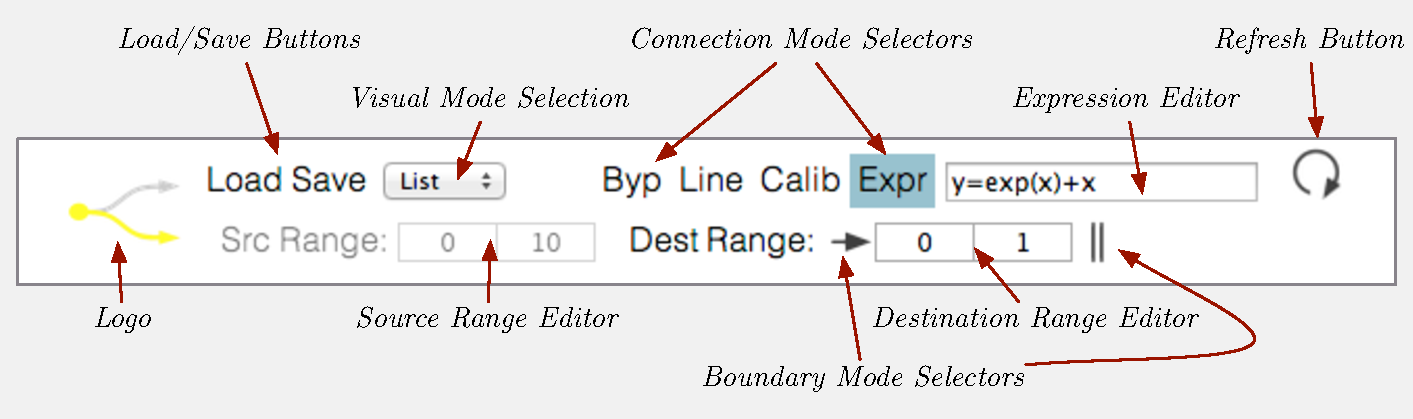
\includegraphics{figures/top_toolbar}}
\caption{The upper toolbar}
\label{fig:toolbar}
\end{figure}

\begin{itemize}
	\item \textbf{Administrative controls}
	\begin{itemize}
		\item\emph{Load/Save buttons}: These elements respond to clicks and save and load mappings, as discussed in section \ref{sec:saving_and_loading}.
		\item\emph{Visual mode selection}: A drop-down menu containing all possible view modes (at the writing of this thesis: List, Grid and Hive).
		\item\emph{Refresh Button}: When clicked, all data residing on the GUI is erased and re-gathered. This is useful if the monitor somehow desynchronizes with the network.
	\end{itemize}

	\item \textbf{Connection modification}
	\begin{itemize}
		\item\emph{Connection mode selectors}: If a single connection is selected within the GUI, this array of buttons allows the user to choose between the available connection modes.
		\item\emph{Expression editor}: Here the user inputs a custom expression, if in ``Expr'' mode, in other modes this field displays the connection's expression but is not editable.
		\item\emph{Source range editor}: These two numbers reflect the maximum and minimum values of the input signal, is only editable in the ``Line'' connection mode.
		\item\emph{Destination range editor}: Same as above but for the destination signal. Due to boundary conditions these fields are useful in all modes.
		\item\emph{Boundary mode selectors}: Two buttons that cycle through five boundary modes for both the maximum and minimum destination value. A graphic exists to represent each mode.
	\end{itemize}
\end{itemize}

All interface features not present in the top toolbar are part of the current visualization mode and are placed into a ``container'' element below, occupying the remainder of the window.

	% subsection top_toolbar (end)

	\subsection{Grid \& Hive views} % (fold)
	\label{sec:grid_&_hive_views}

\begin{figure}[ht]
\centering
	\scalebox{0.4}{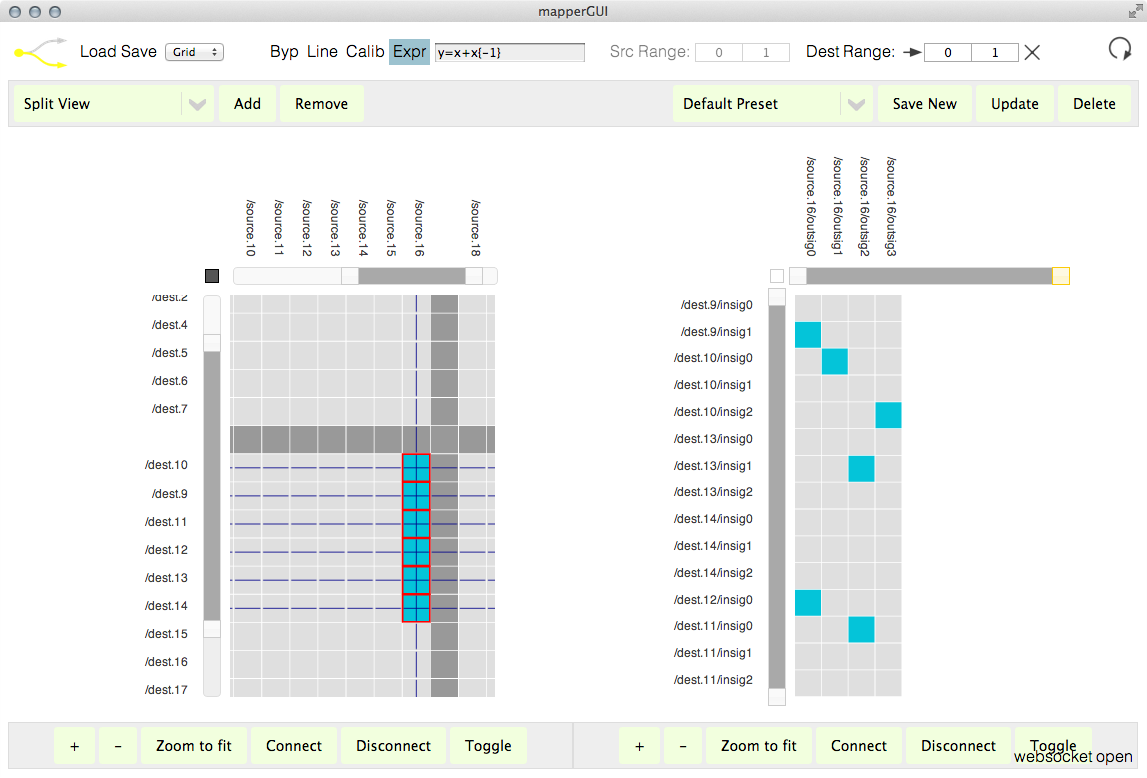
\includegraphics{figures/grid}}
\caption{The grid view}
\label{fig:grid}
\end{figure}

\begin{figure}[ht]
\centering
	\scalebox{0.4}{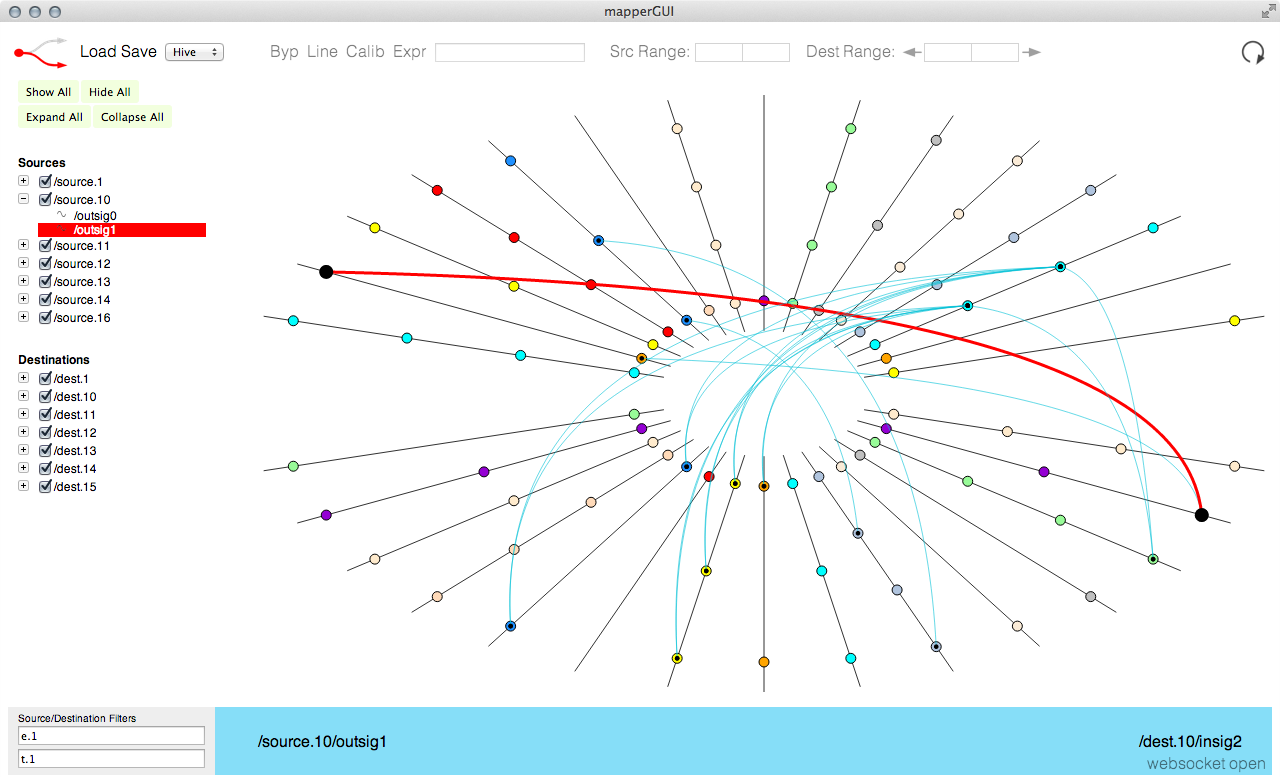
\includegraphics{figures/hive}}
\caption{The hive view}
\label{fig:hive}
\end{figure}
	
	% subsection grid_&_hive_views (end)

%%%%%%%%%%%%%%%%%%%%%%%%%%%%%%%%%%%%%%%%%%%%%%%%%%%%%%%%%%%%%%%%%%%%%%%%%%%%%%%%%%%%%%%%%%%%%%%%%%%%%%%%%%%%%%%%%%%%%%%%%%%%%%%%%%%%%%%%%%%%%%%%%%%%%%%%%%%%%%%%%%%%%%%%%%%%%%%%%%%%%%%%%%%%%%%%%%%%%%%%%%%%%%%%%%%%%%%%%%%%%%%%%%%%%%%%%%%%%%%%%%%%%%%%%%%%%%%%%%
\section{Other GUI Features}

	\subsection{Saving \& Loading} % (fold)
	\label{sec:saving_and_loading}
	
	% subsection saving_&_loading (end)

	\subsection{Creation of a standalone \& distribution} % (fold)
	\label{sec:creation_of_a_standalone_and_distribution}
	
	% subsection creation_of_a_standalone_&_distribution (end)


\subsection{List view}
\label{sec:list_view}


The first implemented, and thus far most functional view mode for the GUI is the ``list'' view. Based heavily on the Max/MSP GUI described in section \ref{sec:similar_interfaces}, the list view provides the most straightforward way to visualize and interact with libmapper. Two tables dominate the visible area, listing source elements on the left and destination elements on the right. B\'ezier curves form lines between associated list elements on each each list. Because these curves do not always represent the same data structures, the lines themselves are referred to as \emph{arrows} by the GUI code, and by this document.

\begin{figure}[ht]
\centering
	\scalebox{0.4}{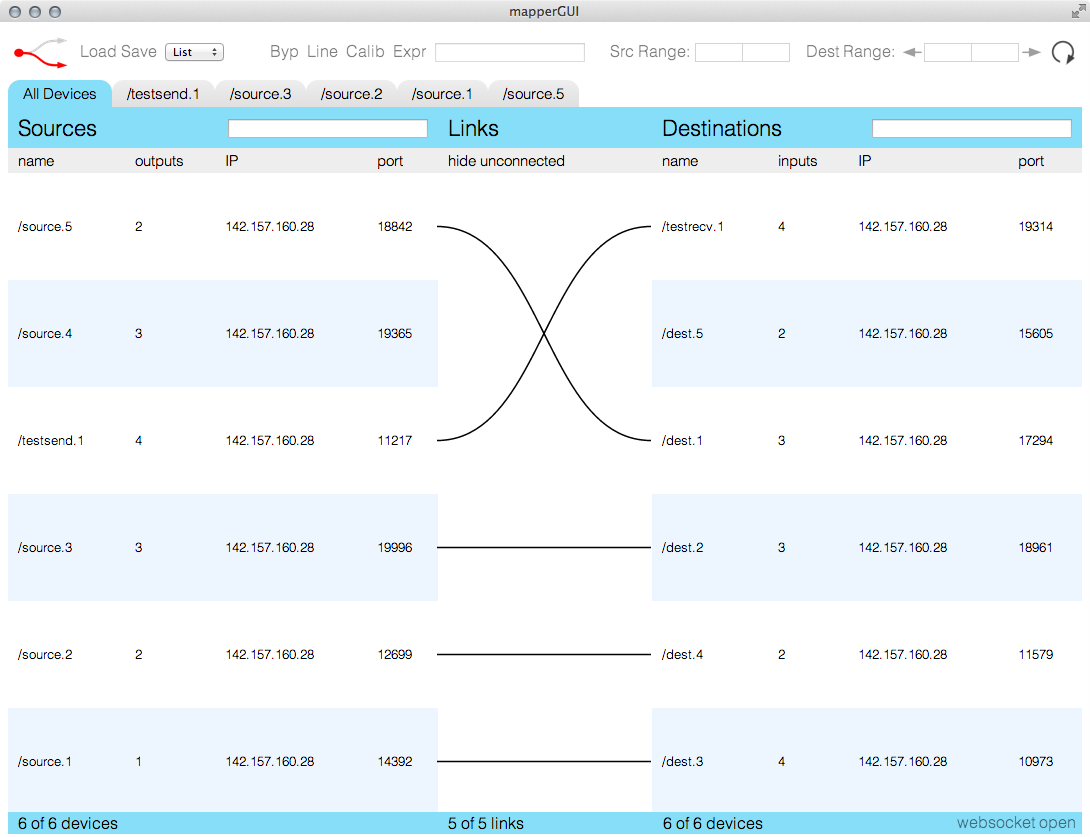
\includegraphics{figures/list_view_all_devices}}
\caption{The list view with all devices selected}
\label{fig:list_view_all_devices}
\end{figure}

The view itself is divided into two major modes: ``All Devices'' and individual linked source devices. Switching between these modes is accomplished through tabs that appear at the top of the container, much like the tabs that appear in modern web browsers. In the All Devices tab, every device displayed on the network is listed in one of the two columns, as in \ref{fig:list_view_all_devices}. Source devices are listed in the left table, while the right table lists destination devices. Intermediate devices, such as implicit mappers described in \cite{interpolated_mappings}, will be listed in both tables. Here arrows represent links between devices. Currently the GUI provides users with names, the number of child signals, IP addresses and a port for every device. Since no connections or signals are displayed, most of the top bar is disabled in the All Devices tab. Saving and loading is also disabled.

\begin{figure}[ht]
\centering
	\scalebox{0.4}{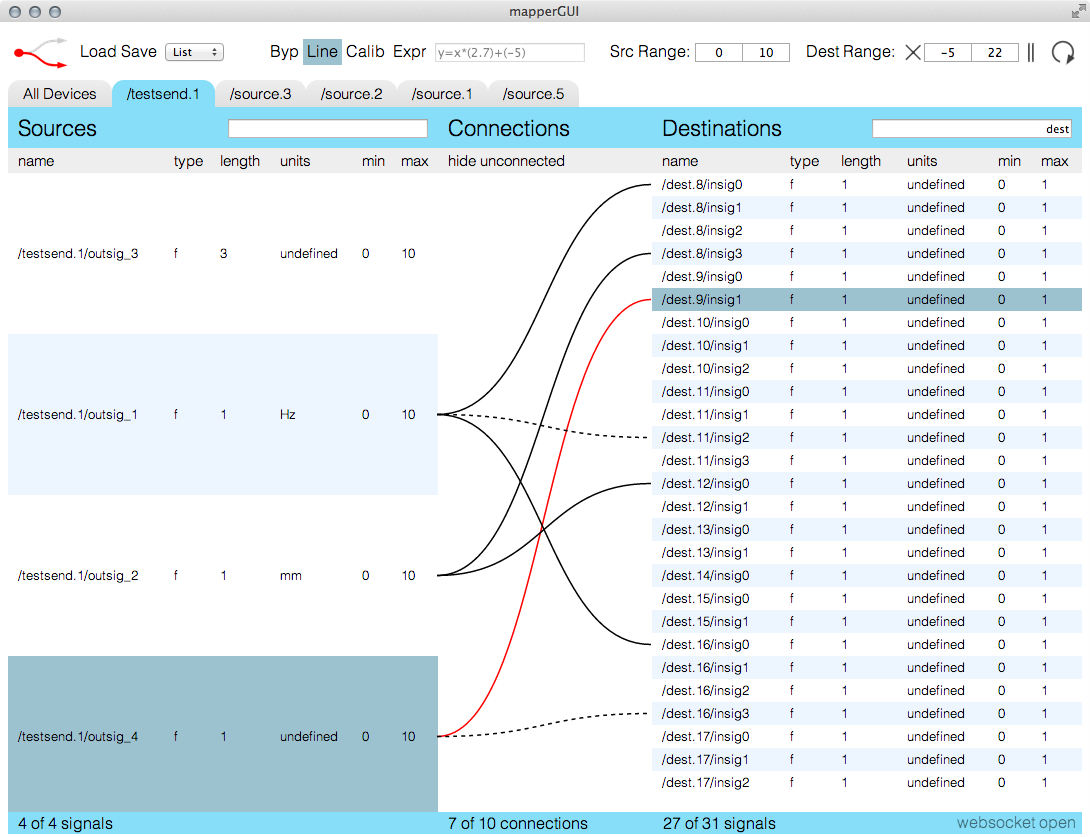
\includegraphics{figures/list_view_single_link}}
\caption{The list view with device \textbf{testsend.1} selected}
\label{fig:list_view_single_link}
\end{figure}

The GUI draws a tab for every source device with at least one link to a destination device. Clicking on any of these devices will redraw both tables. The left table now shows all child signals for the selected source device while the right table displays child signals for every destination device linked to the selected device. 

\begin{figure}[ht]
\centering
	\scalebox{0.4}{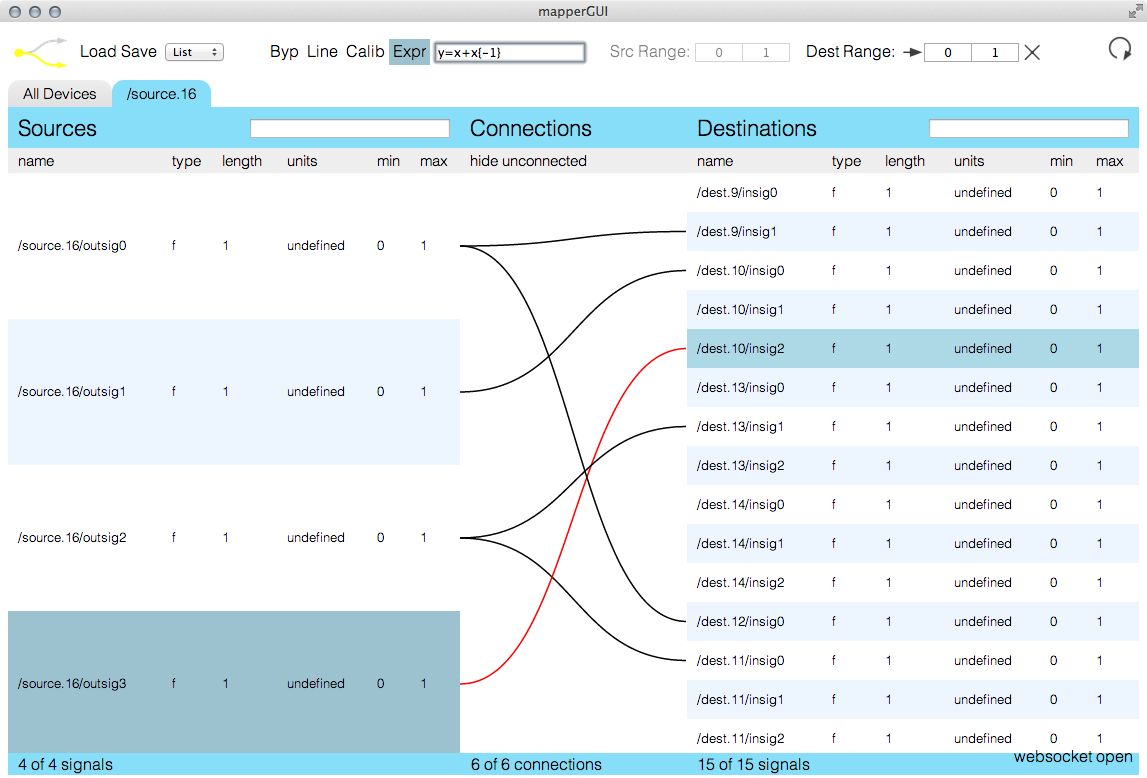
\includegraphics{figures/final_list}}
\caption{The list view after redesign} %TODO before redesign
\label{fig:before_makeover}
\end{figure}


